\documentclass[a4paper, 12pt]{article}
\usepackage[a4paper,top=1.5cm, bottom=1.5cm, left=1cm, right=1cm]{geometry}
\usepackage{cmap}					% поиск в PDF
\usepackage{mathtext} 				% русские буквы в формулах
\usepackage[T2A]{fontenc}			% кодировка
\usepackage[utf8]{inputenc}			% кодировка исходного текста
\usepackage[english,russian]{babel}	% локализация и переносы

\usepackage{amsmath,amssymb}
\usepackage{indentfirst}
\usepackage{longtable}
\usepackage{graphicx}
\usepackage{array}
\usepackage{float}

\usepackage{floatflt}
\usepackage{wrapfig}
\usepackage{siunitx} % Required for alignment
\usepackage{subfig}
\usepackage{multirow}
\usepackage{rotating}
\usepackage{caption}

\graphicspath{{.}}

\title{\begin{center}Лабораторная работа №5.5.5\end{center}
Компьютерная сцинтилляционная $\gamma$-спектрометрия}
\author{Рожков А. В.}
\date{\today}

\begin{document}
    \pagenumbering{gobble}
    \maketitle
    \newpage
    \pagenumbering{arabic}

    \textbf{Цель работы:} Снять и исследовать спектры излучения различных источников, характеризовать различные пики в спектрах радиоактивных веществ.

    \textbf{В работе используются:} сцинтиллятор NaI(Tl), ФЭУ, предусилитель импульсов, высоковольтный блок питания для ФЭУ, АЦП, компьютер, осциллограф.

    \section{Теоретическое введение}

        В работе используется сцинтилляционный метод исследования излучений. Основным элементом является сцинтиллятор - вещество, способное излучать видимое или ультрафиолетовое излучение под действием заряженных частиц. Внутри вещества наблюдаются следующие 3 явления:

        \subsection{Фотоэффект}

            Это процесс взаимодействия гамма-кванта с электроном, связанным с атомом, при котором электрону передается вся энергия гамма-кванта.

            Кинетическая энергия электрона равна
            $$
                T_e = Е_\gamma – I_i
            $$
            где $Е_\gamma$ – энергия гамма-кванта, $I_i$ – потенциал ионизации $i$-той оболочки атома.

        \subsection{Эффект Комптона}

            Это упругое рассеяние фотона на свободном электроне, сопровождающееся изменением длины волны фотона (реально этот процесс происходит на слабо связанных с атомом внешних электронах). Максимальная энергия образующихся комптоновских электронов соответствует рассеянию гамма-квантов на $180^o$ и равна

            $$
                E_{\max} = \frac{\hbar\omega}{1 + \frac{mc^2}{2\hbar\omega}}
            $$

        \subsection{Процесс образования электрон-позитронных пар}

            При достаточно высокой энергии гамма-кванта наряду с фотоэффектом и эффектом Комптона может происходить третий вид взаимодействия гамма-квантов с веществом -- образование электрон-позитронных пар.

            Пороговая энергия, необходимая для образования пары:

            $$
                E_{пор} \approx 2mc^2 = 1,022~МэВ
            $$

            При этом возможны три варианта развития событий:

            а) оба родившихся гамма-кванта не вылетают из детектора, и тогда вся энергия первичного гамма-кванта останется в детекторе, а в спектре появится пик с $E = E_{\gamma}$;

            б) один из родившихся гамма-квантов покидает детектор, и в спектре появляется пик, соответствующий энергии $E = E_{\gamma} - E_0$ где $Е_0 = mc^2 = 511 кэВ$;

            в) оба родившихся гамма-кванта покидают детектор, и в спектре появляется пик, соответствующий энергии $Е = E_{\gamma} - 2E_0$, где $2Е_0 = 2mc^2 = 1022 кэВ$.

        Таким образом, любой спектр, получаемый с помощью гамма-спектрометра, описывается несколькими компонентами, каждая из которых связана с определенным физическим процессом.

        Помимо этих процессов, добавляются экспонента, связанная с наличием фона, пик характеристического излучения, возникающий при взаимодействии гамма-квантов с окружающим веществом, а также пик обратного рассеяния, образующийся при энергии квантов $E_{\gamma} \gg mc^2$ в результате рассеяния гамма-квантов на большие углы на материалах конструктивных элементов детектора и защиты и последующего фотоэффекта в сцинтилляторе. Положение пика обратного рассеяния определяется по формуле:

        $$
            E_{обр} = \frac{E}{1 + 2E/mc^2}
        $$
        где $E$ -- энергия фотопика

        \subsection{Энергетическое разрешение спектрометра}

            Даже при поглощении частиц с одинаковой энергией амплитуда импульса на выходе фотоприёмника сцинтилляционного детектора меняется от события к событию. Это связано:

            1)~со статистическим характером процессов сбора фотонов на фотоприёмнике и последующего усиления,
            2)~с различной вероятностью доставки фотона к фотоприёмнику из разных точек сцинтиллятора,
            3)~с разбросом высвечиваемого числа фотонов.

            В результате в экспериментальном спектре линия (которая для идеального детектора представляла бы дельта-функцию) оказывается размытой, её часто описывают гауссианом.

            Энергетическим разрешением спектрометра называется величина
            $$
                R_i = \frac{\Delta E_i}{E_i},
            $$
            где $\Delta E_i$ -- ширина пика полного поглощения, измеренная на половине высоты (в единицах энергии), $E_i$ -- энергия регистрируемых гамма-квантов. Значение $E_i$ пропорционально среднему числу фотонов $\bar{n_i}$ на входе ФЭУ:
            $$
                E \propto \bar{n}.
            $$

            Полуширина пика $\Delta E_i$ пропорциональна среднеквадратичной флуктуации $\bar{\Delta n_i}$. Так как $n_i$ распределено по закону Пуассона, то $\bar{\Delta n_i} = \sqrt{\bar{n_i}}$ и поэтому
            $$
                \Delta E_i \propto \sqrt{\bar{n_i}}.
            $$

            Из вышесказанного получаем:
            $$
                R_i = \frac{\Delta E_i}{E_i} \propto \frac{1}{\sqrt{E_i}}.
            $$
            Таким образом, чем выше энергия гамма-кванта, тем меньше разрешение.

        \subsection{Форма импульсов}

            Схема ФЭУ представлена на рисунке \ref{img:FEU}

            \begin{figure}[h!]
                \begin{center}
                    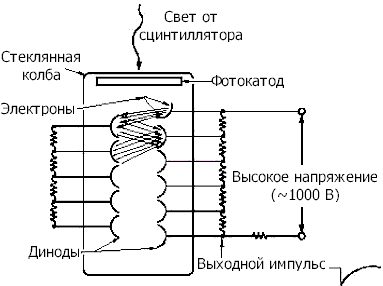
\includegraphics[width = 0.5\textwidth]{img/FEU.png}
                    \caption{Схема ФЭУ}
                    \label{img:FEU}
                \end{center}
            \end{figure}

            Сигнал на выходе имеет вид:
            $$
                U(t) \propto e^{-t/RC}(1 - e^{-t/\tau_0}
            $$
            где $\tau_0$ -- время высвечивания сцинтиллятора, а $RC$ -- постоянная времени, определяемая анодной цепью ФЭУ.

            Чтобы сигнал было удобно регистрировать, $RC$ выбирают много больше, чем $\tau_0$.

    \section{Экспериментальная установка}

        \begin{figure}[h!]
            \begin{center}
                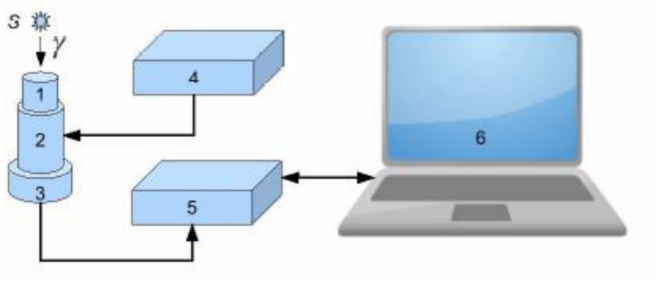
\includegraphics[width = 0.5\textwidth]{img/ust_labnik.png}
                \caption{Принципиальная блок-схема спектрометра. (1 – сцинтиллятор, 2 – ФЭУ, 3 – предусилитель импульсов, 4 – высоковольтный блок питания для ФЭУ, 5 – блок преобразования аналоговых импульсов с ФЭУ в цифровой код (АЦП), 6 – компьютер для сбора данных, их обработки и хранения).}
                \label{img:ust_labnik}
            \end{center}
        \end{figure}

        \begin{figure}[h!]
            \begin{center}
                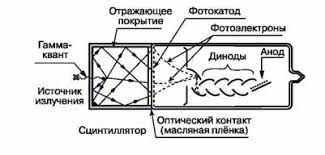
\includegraphics[width = 0.5\textwidth]{img/ust.jpg}
                \caption{Пример схематического устройства сцинтилляционного детектора}
                \label{img:ust}
            \end{center}
        \end{figure}

        Исследуемое излучение попадает на вещество-сцинтиллятор. Вещество представляет собой неорганический кристалл NaI(Tl). Для предотвращения сильного поглощения излучения в сцинтилляторе вводят небольшие добавки других атомов (в данном случае атомы Таллия). Свободные локальные уровни энергии электрона на примесных атомах таллия располагаются внутри запрещенной зоны кристалла NaI.
        В процессе релаксации возможны переходы электронов, возбужденных в зону проводимости, на эти уровни. Энергии излучаемых при таких переходах фотонов меньше ширины запрещенной зоны, и они могут поглощаться только атомами таллия. Но концентрация таллия мала (порядка $0,1\%$), поэтому мало поглощение указанных фотонов, и они имеют все шансы вылететь из сцинтиллятора. В этом случае прохождение ионизирующей частицы через вещество будет сопровождаться световой вспышкой, которая и может быть использована для регистрации частицы.

        Испущенный сцинтиллятором свет попадает на фотокатод и выбивает из него электроны, которые далее умножаются при помощи ФЭУ. На каждом уровне динодов один электрон выбивает несколько новых, образуя лавину. В конечном итоге электроны попадают на анод. При помощи предусилителя импульсов и АЦП сигнал регистрируется компьютером.

    \section{Ход работы}



\end{document}
